\documentclass[12pt]{ruthesis}
%\documentclass[12pt]{amsart}
\usepackage{amsmath}
\usepackage{amssymb}
\usepackage{latexsym}
\usepackage{epsfig,epsf,rotating}
\usepackage{subfigure}
\usepackage{siunitx}
%\usepackage{pictex}
\usepackage{epsf}
\usepackage{theorem}
\usepackage{graphicx}
\usepackage{hyperref}
\usepackage{typedref}
\usepackage[version=4]{mhchem}
%\usepackage{cite}
\usepackage[numbers, sort&compress]{natbib}

\title{Microwave spectroscopy on two dimensional electron gas}
\ctitle{Microwave spectroscopy on two dimensional electron gas}
\author{Jie Zhang}
\department{Physics and Astronomy}
\school{Rice University}
\degree{Master of Science}

\committee {
		Rui-Rui Du, Chair\\
        Professor of Physics and Astronomy \and
        Junichiro Kono \\
        Professor of Electrical and Computer Engineering and Physics \& Astronomy \and
        Wei Li\\
        Associate Professor of Physics and Astronomy\and
       }

\address{Houston, Texas}
\donemonth{August} \doneyear{2015} \makeindex
\begin{document}

  \begin{frontmatter}
   \pagenumbering{roman}
   %\makecover
   \maketitle

\begin{abstract}

Electron spin resonance (ESR) and cyclotron resonance (CR) are two of the most significant feature of electrons under magnetic field.
In order to detect the ESR of a single nano-object, a highly sensitive tool is required.
So far, the best commercial ESR detector can detect around 1000 spins.
We develop an ultra-sensitive calorimeter which is aimed at resolving the ESR of one nano-object.
This nano-calorimeter can operate at \SI{300}{\milli\kelvin} and the precision is improved to tens of micro-Kelvins, thereby increasing the sensitivity to several nano-watts.
As a proof of concept, we show that CR can be measured via heat generated by resonant absorption of photons using this setup.
An increase in the lattice temperature can be detected when the energy of the incident microwave photons matches the energy difference between adjacent Landau levels, and cannot be detected at other frequencies.

We constructed another setup to investigate edge state transport.
Microwave absorption spectroscopy of quantum droplets in a two dimensional electron gas (2DEG) is a powerful tool for investigating the number and velocities of the charge modes.
We have sample patterned with multiple circular dots on the order of several microns.
It is directly placed onto the meander line superconducting waveguide positioned inside a resonance container.
The whole setup is attached to the bottom of a top loaded \ce{^{3}He} cryostat with base temperature down to \SI{300}{\milli\kelvin}.
This absence of a contact gives this setup an advantage over standard transport measurements and could be generalized to a standard method for probing edge states hosted in other new materials.


\end{abstract}

%\include{ack}
\tableofcontents
\listoffigures
%\listoftables
%   \include{ded}
\end{frontmatter}
\pagenumbering{arabic}
\linespacing{1.7}



\chapter{Transport behavior of electrons under the illumination of microwave}\label{Transport}

\section{Shubnikov-de Haas oscillations}\label{SdHO}
When a magnetic field is applied to an ideal 2DEG, the constant density of states breaks into isolated delta functions with a spacing of $\hbar\omega_{c}$, where $\omega_{c}: =\frac{eB}{m^{*}}$ is the cyclotron frequency.
In a real 2DEG, these delta functions are broadened (but not shifted) into Lorentzian functions
\begin{align}
L(E) := \frac{1}{\pi} \frac{\Gamma/2}{(E - E_{LL})^{2} + (\Gamma/2)^{2}}
\end{align}
due to scattering mechanisms.
The peaks $E_{LL}$ of these Lorentzians are called Landau levels and have a full width at half maximum (FWHM) of $\Gamma=\hbar/\tau q$ where $q$ is the quantum lifetime, \emph{i.e.\!} the mean time between two scattering events.
In order to resolve the peak, the magnetic field must be strong enough that $\hbar\omega_{c}\gg \Gamma$ or $\omega_{c}\tau q \gg 1$.
Heuristically we understand this condition as meaning that an average electron is be able to undergo at least one cyclotron orbit without scattering.

The areal density of states in each Landau level denoted by $n_{B} :=\frac{eB}{h}$ giving a filling factor of $\nu =\frac{n_{2D}}{n_{B}}=\frac{h}{eB}n_{2D}$.
Therefore, when the Fermi energy $E_{F}$ lies precisely between two separate Landau levels, longitudinal conductance reaches a local minimum and attains a local maximum when $E_{F}$ lies on a peak.
As the magnetic field pushes the Fermi energy through adjacent Landau levels, the longitudinal resistance $R_{xx}$ rises and falls, giving rise to the well-known \emph{Shubnikov-de Haas oscillations} (\figureref{sdho}).

\begin{figure}[!htb]\centering
   \begin{minipage}{0.49\textwidth}
     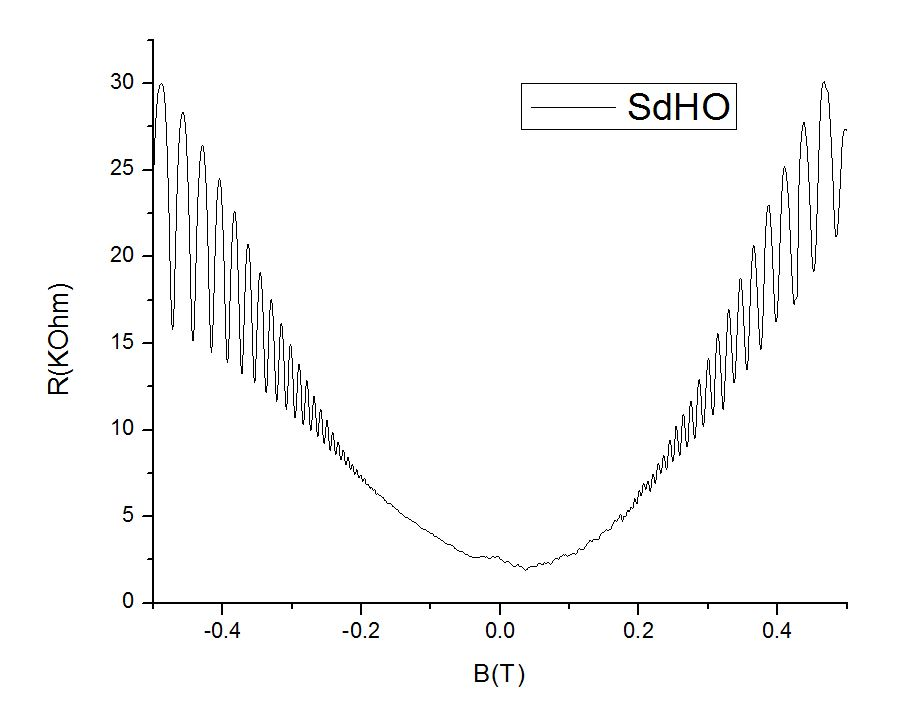
\includegraphics[width=\linewidth]{figures/sdho.JPG}
     \caption{Shubnikov-de Haas oscillations}\label{sdho}
   \end{minipage}
   \begin {minipage}{0.49\textwidth}
     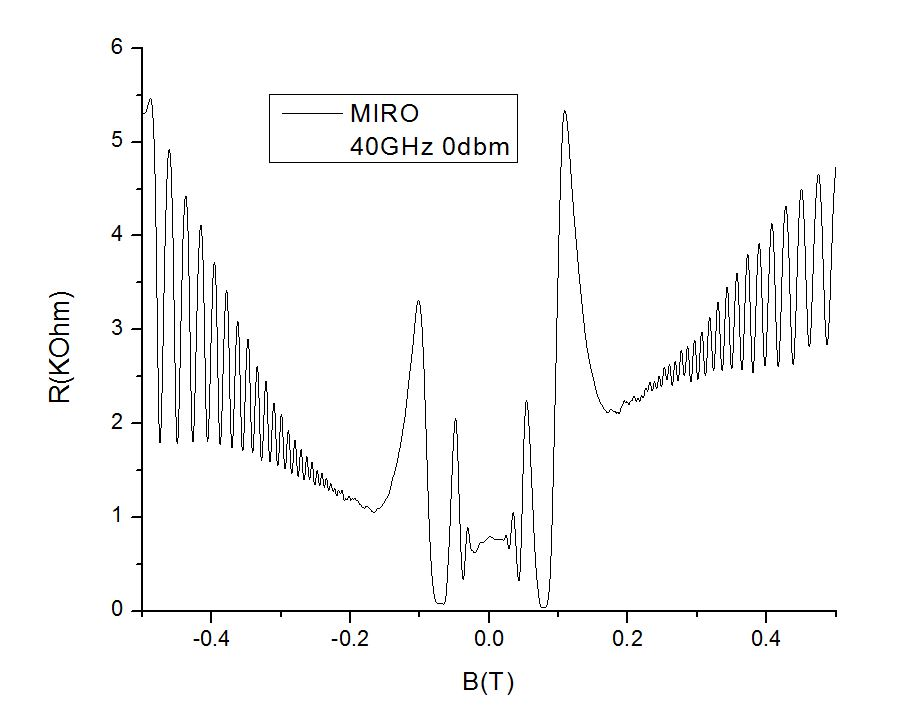
\includegraphics[width=\linewidth]{figures/miro.JPG}
     \caption{Microwave Induced Resistance Oscillations}\label{miro}
   \end{minipage}
\end{figure}





\section{Microwave induced resistance oscillations}\label{MIRO}

When a microwave field is applied, \figureref{sdho} changes quite dramatically.
Additional maximums appear with different intensity at different peaks which is known as microwave induced resistance oscillations (MIRO), see \figureref{miro}.
MIRO is fascinating nonequilibrium transport phenomenon found in both n-type and p-type ultrahigh mobility 2D systems. 


 
Theoretical explanations of MIRO involve both a displacement mechanism and an inelastic mechanism \cite{PhysRevB.89.125401}.
Both these mechanisms modify the scattering of electrons due to microwave assistance. This theory predicts that the photoresistance oscillates as
\begin{align}
\delta R_{\omega}/R_{0} =-2\pi\eta P\lambda^{2}\epsilon \sin(2\pi\epsilon)
\end{align} 
where $\eta$ is the dimensionless scattering rate, $P$ is the dimensionless microwave power, $\lambda$ is the Dingle factor which is related to the quantum lifetime as well as cyclotron frequency and $\epsilon :=\omega/\omega_{c}$. 



\chapter{Thermal detection on behavior of electrons under the illumination of microwave}\label{Thermal}





\section{Theoretical support and preparation in \SI{4}{K}}\label{Theoretical}

The density of states of a 2DEG forms Landau levels when a magnetic field is applied.
However, sweeping either microwave frequency or magnetic field will result in the case where energy of the incident photons is equal to the energy gap of the Landau levels, therefore causing resonance.
However, in \ce{AlGaAs/GaAs} material, electron relaxation can be non-radiative by passing the extra energy to phonons and raising lattice temperature.
This temperature change can be measured by a nano-calorimeter.
We constructed such a device using a special Cernox thermometer which has a huge resistance difference for a tiny temperature change at low temperature.

\begin{figure}[!htb]\centering
   \begin{minipage}{0.49\textwidth}
     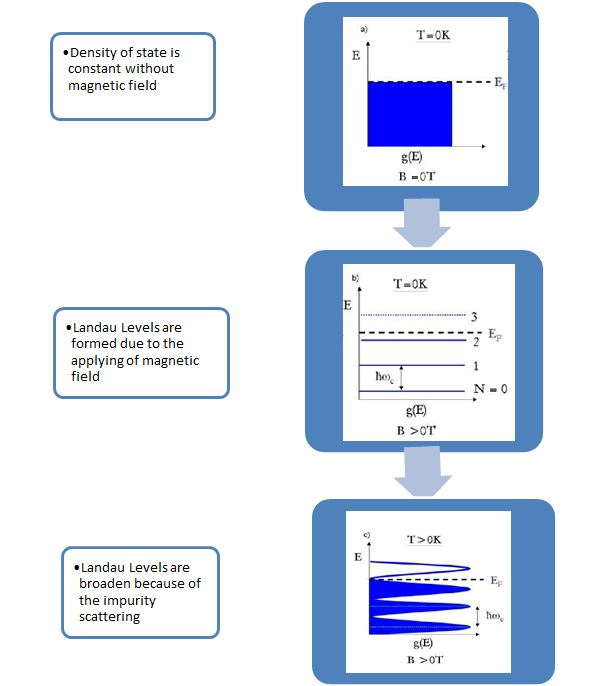
\includegraphics[width=\linewidth]{figures/llformation.JPG}
     \caption{Formation of Landau Levels}\label{llformation}
   \end{minipage}
   \begin {minipage}{0.49\textwidth}
     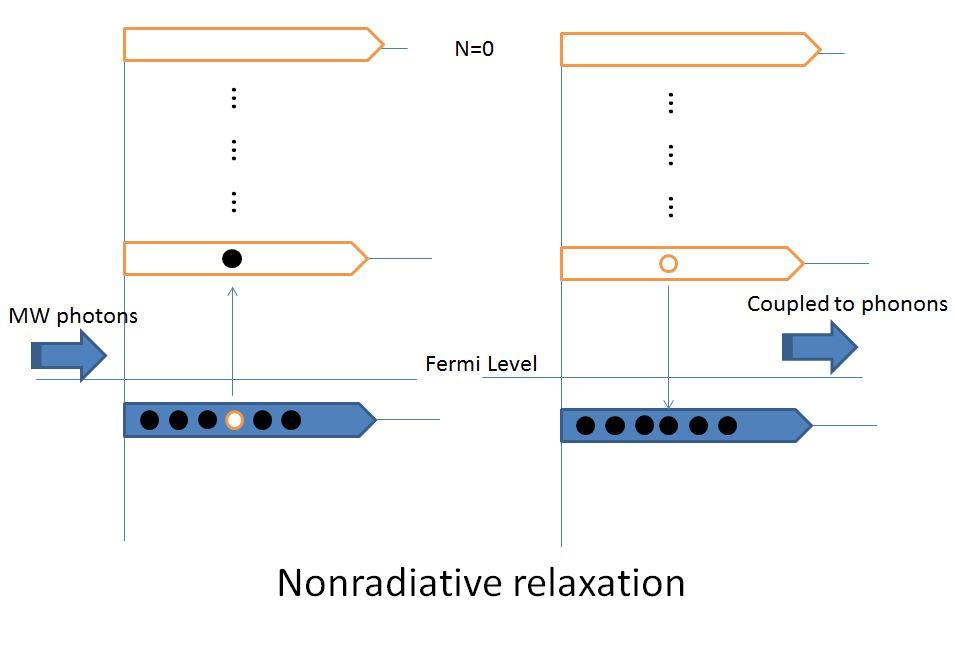
\includegraphics[width=\linewidth]{figures/nonradiative.JPG}
     \caption{Non-radiative relaxation}\label{nonradiative}
   \end{minipage}
\end{figure}

This resonance measuring method has been tested in our group with liquid helium for detecting geometric resonance which is the coupling between cyclotron resonance and plasma resonance. 
On a bare 2DEG chip, cyclotron resonance dips can be resolved clearly.


However, on a patterned sample (with a feature size on the order of \si{\micro\meter}), one can observe two obvious resonances at
\begin{align}
\omega_{\pm}=\frac{\omega_{c}}{2} \pm \sqrt{ \omega_{0}^{2}+ \left(\frac{ \omega_{c} }{2}\right)^{2}},
\end{align}
where $\displaystyle \omega_{0}^{2}=\frac{N_{s}e^{2}}{2m^{\ast}\epsilon_{\mathrm{eff}}r}$, effective mass $m^{*}=0.067m_{e}$, $\epsilon_{\mathrm{eff}}=6.5$ and $r$ is the radius of the dots. 
%In our sample, the electron density $N_{s}=\SI{2.5e11}{\centi\meter^{-2}}$, 
\begin{figure}[!htb]\centering
   \begin{minipage}{0.49\textwidth}
     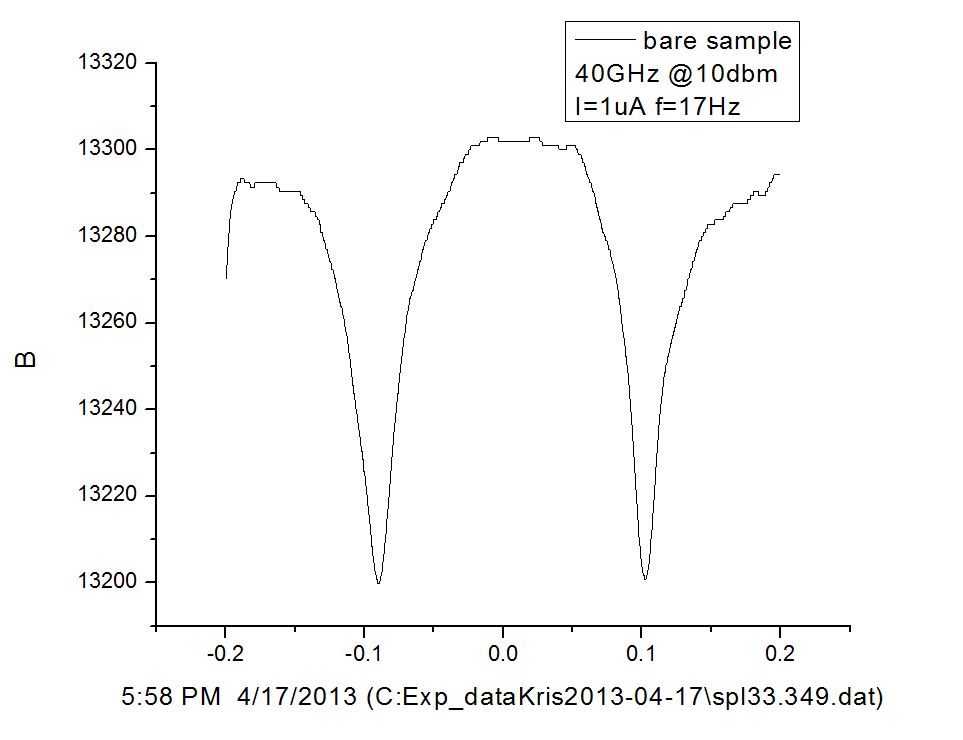
\includegraphics[width=\linewidth]{figures/bare_cr.JPG}
     \caption{Bare chip CR}\label{bare_cr}
   \end{minipage}
   \begin {minipage}{0.49\textwidth}
     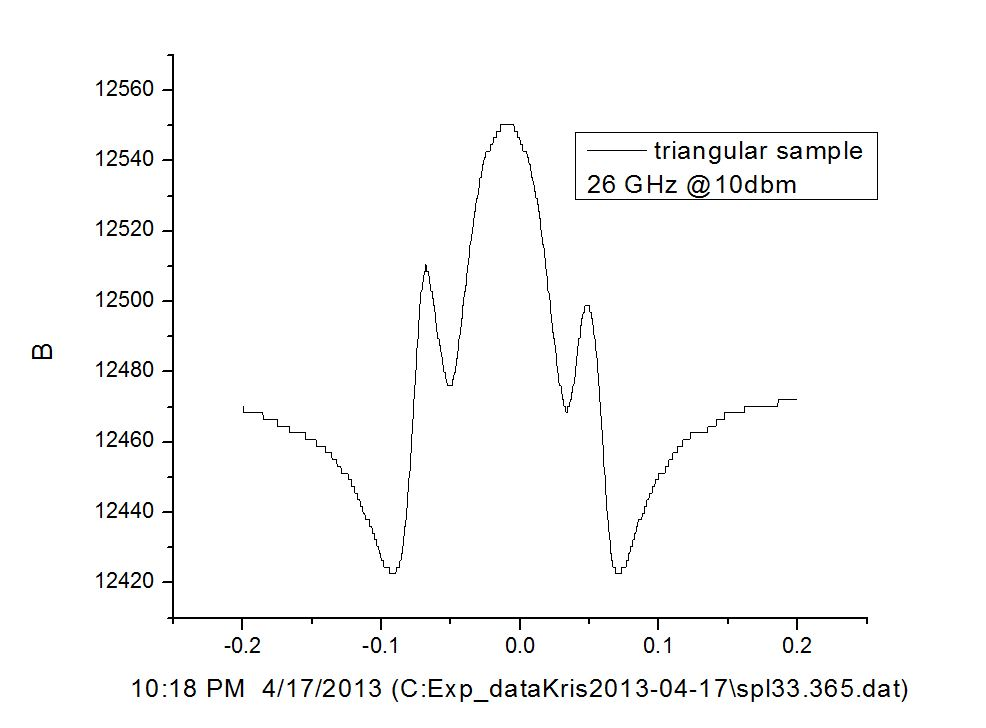
\includegraphics[width=\linewidth]{figures/coupled_cr.JPG}
     \caption{Coupled GR}\label{coupled_cr}
   \end{minipage}
\end{figure}




\cite{PhysRevB.28.4875}

Boundary plasmon has been eliminated by choosing irregularly shaped samples and frequency is limited by the size of our waveguide though it could be extended using frequency multiplier and replacing with coaxial cable. 

 
\section{Setup construction}\label{Construction}

In order to improve the sensitivity, we constructed another setup which works in \SI{300}{\milli\kelvin} due to the fact that the lower the temperature gets, the shaper resistance line the Cernox thermometer's resistance will act (\figureref{r(t)}).

\begin{figure}[!htb]\centering
   \begin{minipage}{0.49\textwidth}
     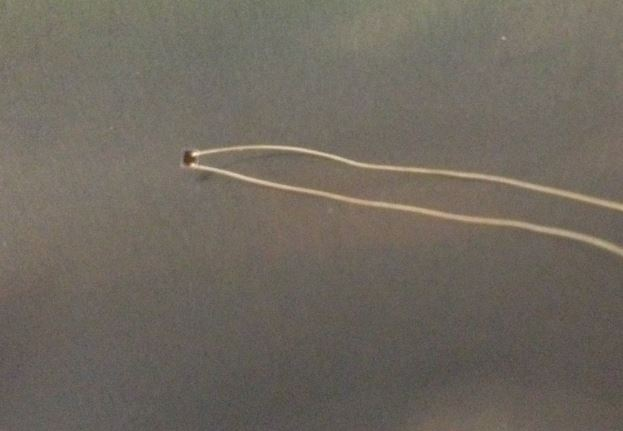
\includegraphics[width=\linewidth]{figures/thermometercx.JPG}
     \caption{Cernox Thermometer}\label{thermometer}
   \end{minipage}
   \begin {minipage}{0.49\textwidth}
     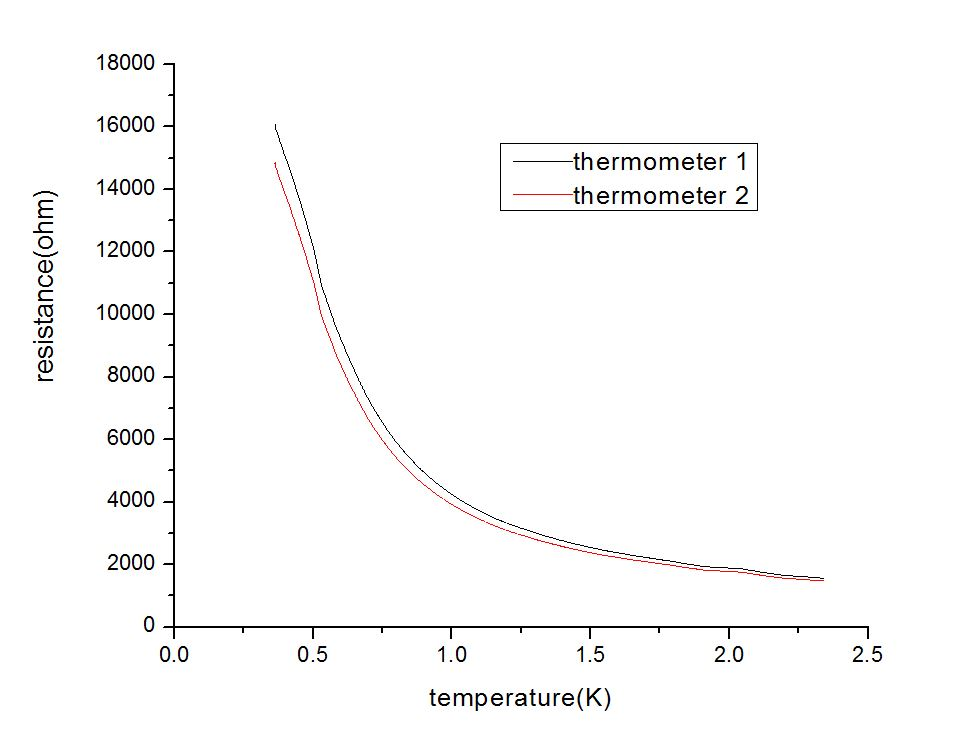
\includegraphics[width=\linewidth]{figures/R(T).JPG}
     \caption{Temperature dependence of the thermometer}\label{r(t)}
   \end{minipage}
\end{figure}
 
 
However, going from \SI{4}{\kelvin} to \SI{300}{\milli\kelvin} is a big leap and there are problems that we have to overcome.
The most significant one is sealing in \ce{^{3}He} liquid environment.
Since the heat generated by the non-radiative relaxation is very small, the sample need to be in vacuum to avoid being carried away by massive \ce{^{3}He} liquid and a high heat conductive media to pass the temperature change to the thermometer.
Meanwhile, to keep the temperature around \SI{300}{\milli\kelvin}, we need something with low heat conductivity to connect the inside setup to outside.
In this case, we use thin sapphire crystal as the bridge between sample and thermometer, thin magnin wire for keeping vacuum temperature low.
Sealing in \ce{^{3}He} liquid environment is hard due to the fact that it's molecules are so small that they'll just enter every tiny gap.
The way we used to seal is tapping the inner wall of the cap and outer wall of the base therefore compressing the flat surfaces of those two parts to seal.
But this is still not enough since the surfaces are polished mechanically only.
We dissolve soap in glycerin and then scribble it on the surfaces to fill up any possible tiny gap.
Validation of the sealing can only be tested by whether the CR signal is resolved.

The whole vacuum can is immersed in liquid \ce{^{3}He} in a top-loaded refrigerator.
Microwaves are sent through a self-made antenna which is connected to the coaxial cable in the probe (see \figureref{probe} and \figureref{thermal-schema}).

\begin{figure}
  \centering
  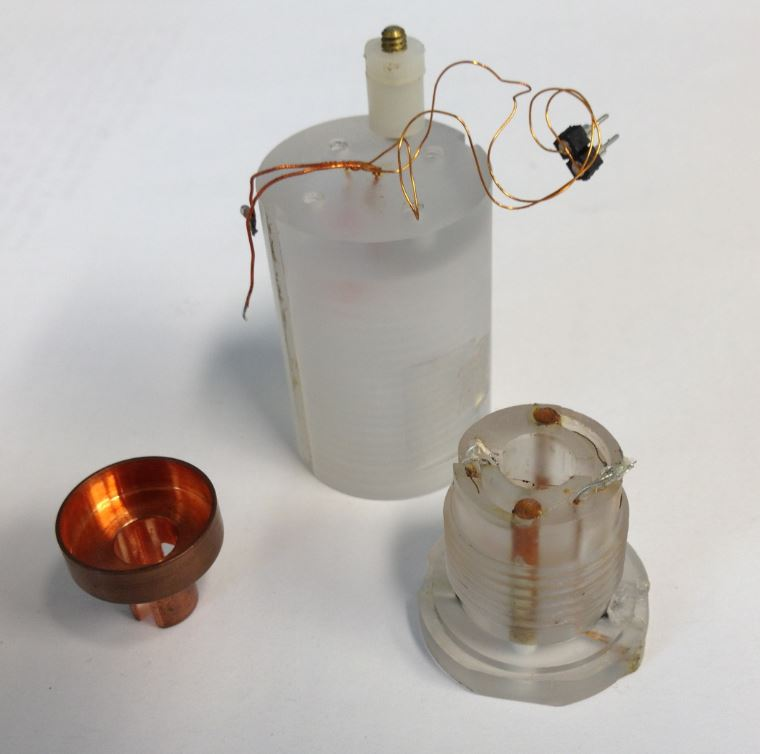
\includegraphics[scale=0.25]{figures/vacuumcan.JPG}
  \caption{1266 Epoxy vacuum can}
  \label{vacuum-can}
\end{figure}
 
 

\begin{figure}[!htb]\centering
   \begin{minipage}{0.49\textwidth}
     \includegraphics[width=\linewidth]{figures/SCHEMA.JPG}
     \caption{Thermal detection setup schema}\label{thermal-schema}
   \end{minipage}
   \begin {minipage}{0.49\textwidth}
     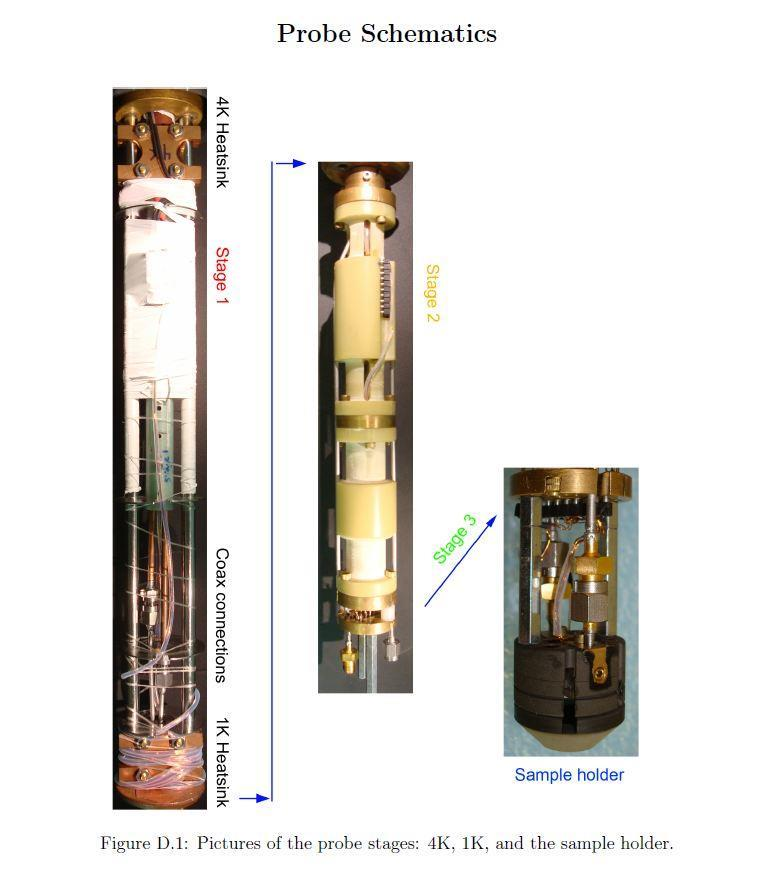
\includegraphics[width=\linewidth]{figures/probe.JPG}
     \caption{\ce{^{3}He} top loaded Refrigerator coaxial probe}\label{probe}
   \end{minipage}
\end{figure}

[from Dr. Kristjan Stone, Ph. D thesis, Millimeter Wave Transmission Spectroscopy of 2D Electron and Hole Systems] 

\section{Cyclotron resonance pretest}\label{Cyclotron}


 
We used a differential circuit to filter the background noise and amplitude modulation technique to quench the asymmetry left in the differential geometry.
The voltage signal difference from the two arms can be calculated by
\begin{align} 
\frac{|\tilde{E}|}{|\tilde{V}|}=\frac{j \omega_{0}(M+L)\delta R}{R^{2}+2j \omega_{0}RL + \omega_{0}^{2} (M^{2}-L^{2})} \approx \frac{\delta R}{2R}
\end{align} 
This indicates that the output signal $V_{\mathrm{out}}$ is linearly proportional to the difference between the resistance of those two Cernox thermometers $\delta R$ which reflects the amount of heat generated by the sample with the illumination of microwave.
The differential signal was fed into the first lock-in amplifier the output of which then was fed into the second lock-in amp. 
The amplitude of the input microwave is modulated internally by the microwave generator according to the frequency of the second lock-in amp which should be much smaller than the rapid oscillating factor of the first lock-in amp. 
Therefore, after integrating twice, the final output should be a clean response of 2DEG CR signal.     
 
\figureref{r(b)} is the response of the thermometer resistance without microwave illumination when magnetic field is swept. There is some irregular response but the result is repeatable. Since the thermometers on the two arms have the same response, by using differential geometry, this influence can be cancelled.
This background indicates that the direction of the magnetic field has asymmetric influence on the two branches. 
\begin{figure}
  \centering
  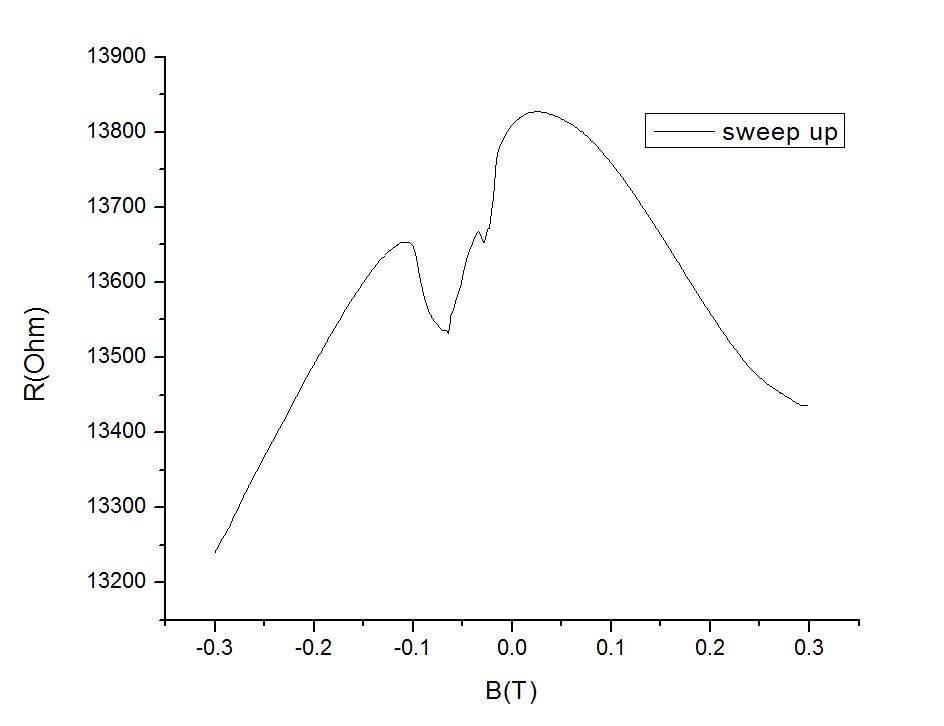
\includegraphics[scale=0.25]{figures/R(B)UP.JPG}
  \caption{Background sweeping}
  \label{r(b)}
\end{figure}

When microwave is applied, obvious resonance peaks appear on each side (see \figureref{0dbm_40ghz}) and the larger the microwave power gets, the higher the resonance peaks shoot. In \figureref{thermopowerdep}, one can see that the signal can still be resolved even with power as low as -20dbm (\SI{0.01}{\milli \watt}). 
Compared to the setup without these two measuring techniques, sensitivity is at least thirty times higher in terms of input microwave power.  



\begin{figure}[!htb]\centering
   \begin{minipage}{0.49\textwidth}
     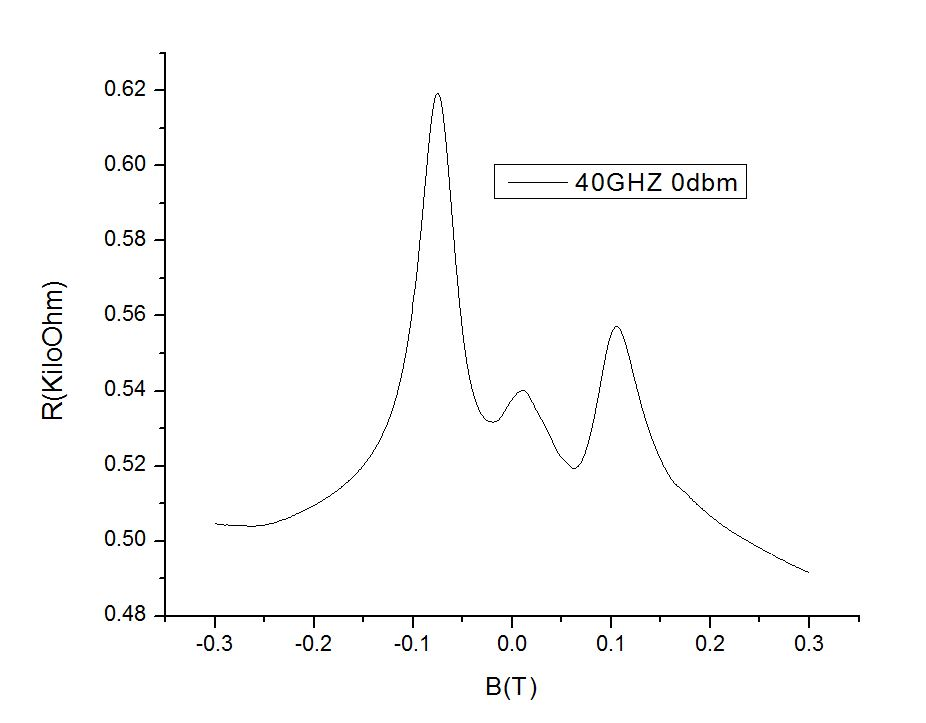
\includegraphics[width=\linewidth]{figures/0dbm.JPG}
     \caption{CR at 0 dbm \SI{40}{\giga \hertz}}\label{0dbm_40ghz}
   \end{minipage}
   \begin {minipage}{0.49\textwidth}
     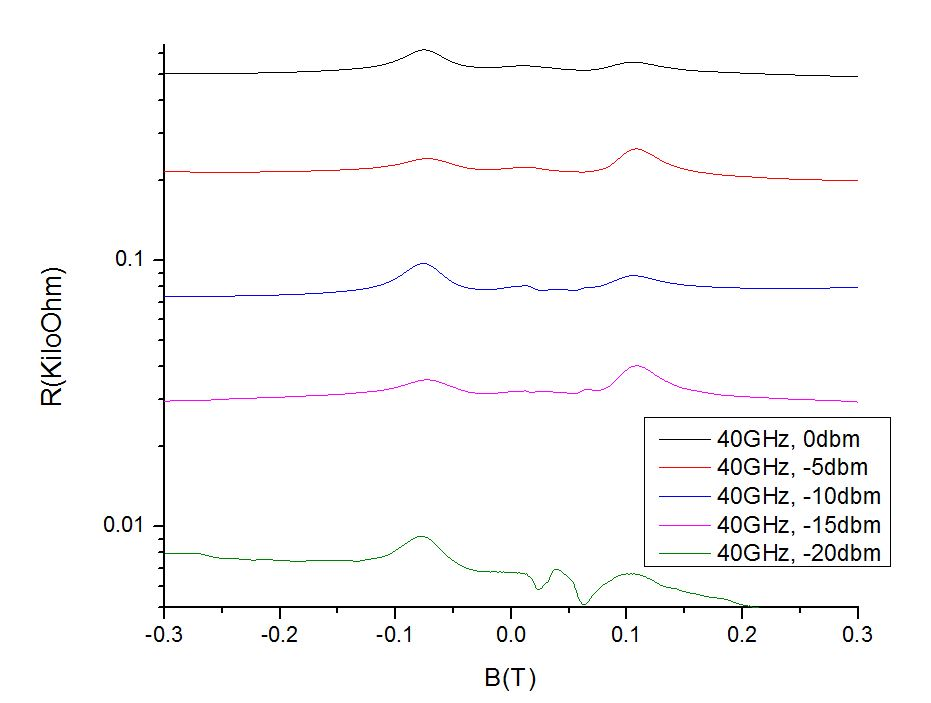
\includegraphics[width=\linewidth]{figures/thermopowerdep.JPG}
     \caption{Power dependence}\label{thermopowerdep}
   \end{minipage}
\end{figure}
 




\section{Spin resonance on DPPH}\label{DPPH}

Electron spin resonance (ESR) or electron paramagnetic resonance (EPR) spectroscopy is a technique for studying materials with unpaired electrons using the Zeeman splitting 
\begin{align}
E=m_{s} g \mu_{B} B_{0}
\end{align}
where $g$ is the electron's Land\'{e} g-factor and $\mu_{B}$ is the Bohr magneton.
Therefore, resonance peak happens at 
\begin{align}
\Delta E=g \mu_{B} B_{0}
\end{align}

The conventional method of measuring ESR is transmission spectroscopy.
There are other ways such as magnetic torque detection, optically detected ESR, STM-ESR and resistively detected ESR which measures the longitudinal resistance of 2DEG. Our thermal detection method is another one by measuring the temperature change induced by the non-radiative relaxation of the photon absorption.

DPPH is a common abbreviation for an organic chemical compound 2,2-diphenyl-1-picrylhydrazyl which has two major applications. One is for monitoring chemical reactions involving radicals while the other is determining the position and intensity of ESR signals. 
In our case, we use dpph to test if ESR signal can be resolved by our setup. 
Raw data is shown in \figureref{dpph_esr} and a clear resonance dip showed up around \SI{1.42}{\tesla} with a line width of 150 Gauss at the microwave frequency of \SI{40}{\giga \hertz}.
Therefore, the g-factor is
\begin{align}
g=\frac{\hbar \omega}{\mu_{B}B}=1.9934
\end{align}
while the theoretical value is the free electron $g=2.0023$.

By subtracting the background and fitting with a Lorentzian (\figureref{dpph_fitting}): 

\begin{align}
L(B)=\frac{A}{[1+ (\frac{\mu g \tau}{h})(B-B_{r})]^{2}}
\end{align}  
we have a decoherence time $\tau = \SI{7.78}{\nano\second}$ which is a reasonable value in our case.

\begin{figure}[!htb]\centering
   \begin{minipage}{0.49\textwidth}
     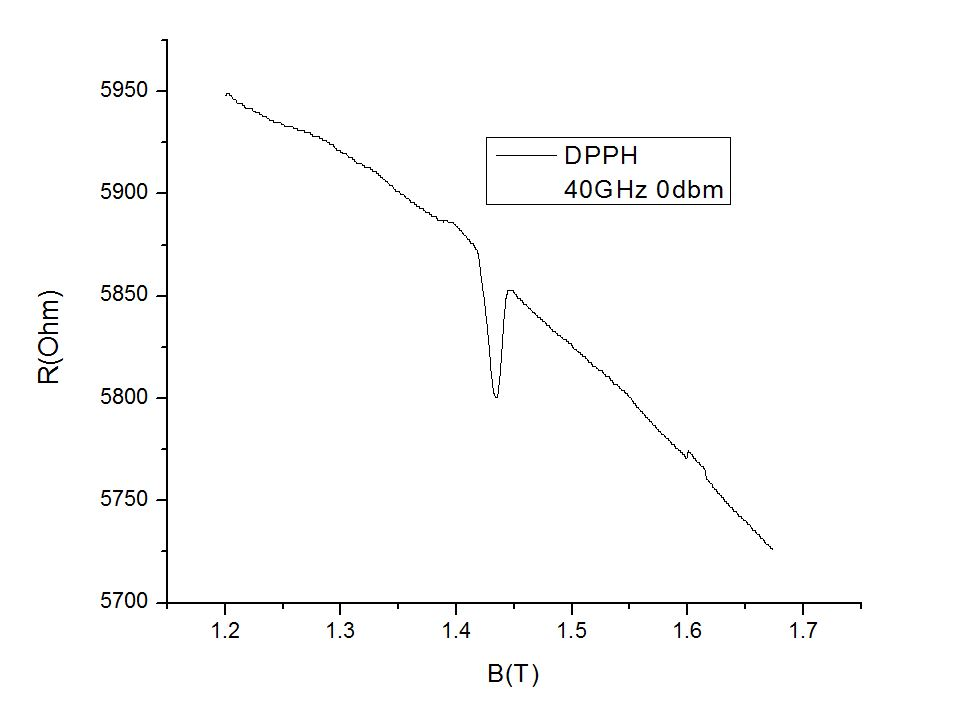
\includegraphics[width=\linewidth]{figures/dpph_esr.JPG}
     \caption{ESR of DPPH}\label{dpph_esr}
   \end{minipage}
   \begin {minipage}{0.49\textwidth}
     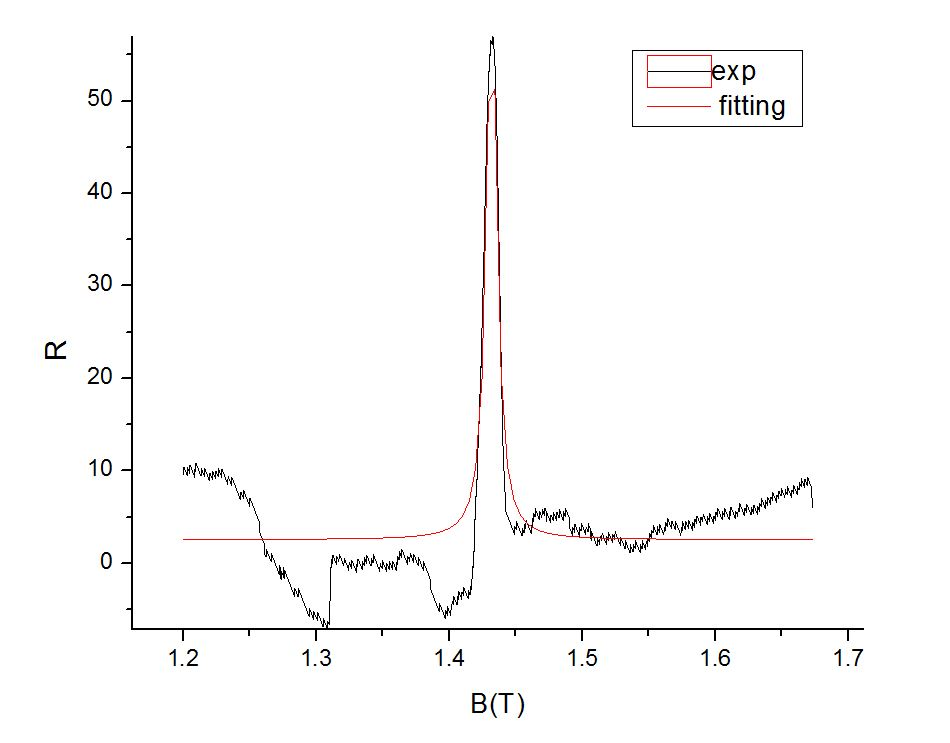
\includegraphics[width=\linewidth]{figures/dpph_fitting.JPG}
     \caption{ESR fitting of DPPH}\label{dpph_fitting}
   \end{minipage}
\end{figure}
 

Here, we demonstrated that the nano-calorimeter we constructed has the ability to resolve both CR and ESR signals for those material which has a non-radiative relaxation process. 








\chapter{Microwave absorption spectroscopy of electrons in 2DEG}\label{Absorption}

This project is aim at investigating the number and velocity of charge modes for edge states on a 2DEG.
With its edge being pure one dimensional and dissipationless, it has tremendous potential applications \cite{PhysRevB.88.165305}.
We patterned high mobility \ce{AlGaAs/GaAs} wafer ($n_{e} \approx \SI{1e11}{cm^{-2}}$, $\mu \approx \SI{15 e6}{\cm^{2}/\volt \second}$) with circular discs with a diameter of several microns by lithography. 
For such a quantum droplet, the minimum energy of the excitations of the edge is $2\pi \hbar \nu /L$. 
The circumference of the droplet is $L=2\pi R$ and the velocity of the charge mode $\nu \approx \SI{1e4}{m/s}$.

To match the microwave energy $\hbar \omega_{M}$, we have 
\begin{align}
\nu = R \omega_{M}
\end{align}
Meanwhile, the velocity of electrons going on cyclotron motion under magnetic field is 
\begin{align}
\nu = 2 f_{c} l_{B}= \frac{2 \omega_{c}}{\pi} l_{B} 
\end{align}
where $\displaystyle \omega_{c}= \frac{eB}{m^{\ast}m_{0}}$ and $\displaystyle l_{B}=\sqrt{\frac{\hbar}{eB}} \approx \frac{257}{\sqrt{B}} \si{\angstrom}$.
Therefore, for electrons in \ce{AlGaAs/GaAs}, the resonant frequency is related to the radius of the disc in the following way:

\begin{align}
R_{e}= \frac{\omega_{x}}{\omega_{M}} \frac{l_{B}}{\pi} \approx \frac{3.4}{\sqrt{B}} \, \si{\micro\meter/\giga\hertz}
\end{align}

By sweeping magnetic field or microwave frequency, we should be able to see a resonant peak with a line width related to the distribution of the disc radius. 


\section{Setup construction and calibration}\label{Construction}

We used a co-plane meanderline waveguide (see \cite{APLBroadbandESR}) to hold the patterned sample then placed the waveguide on the top of a broad band sample holder.
Electrical connection is done by silver paste.  
The sample holder is connected to the coaxial cable in the transmission probe by a mini-SMP connector.
Again, this whole setup is immersed in \ce{^{3}He} liquid in a top-loaded cryostat.


\begin{figure}
  \centering
  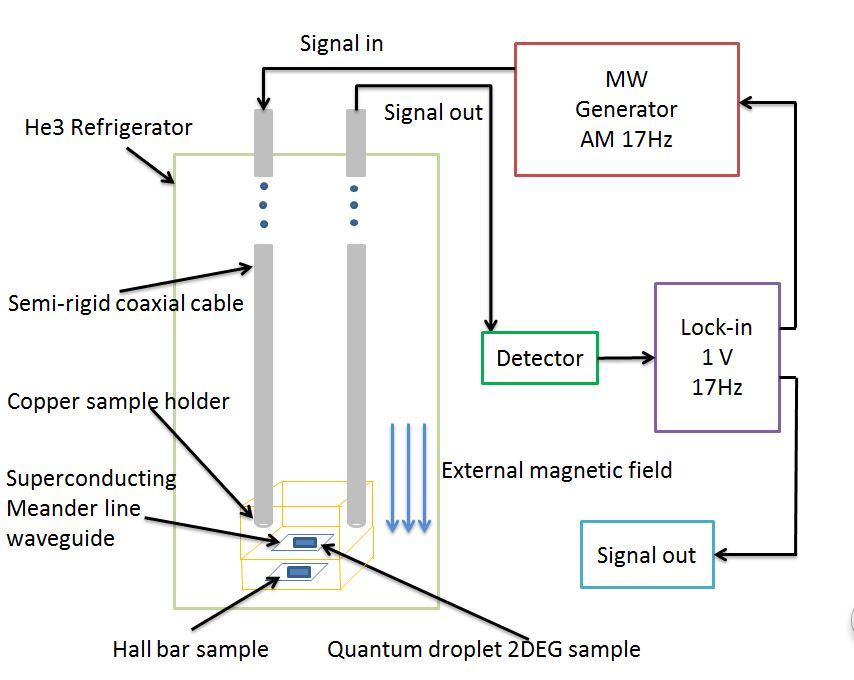
\includegraphics[scale=0.25]{figures/configuration.JPG}
  \caption{Microwave absorption spectroscopy construction}
  \label{configuration}
\end{figure}
 
We used AM modulation at \SI{17}{\hertz} for measuring except this time, the output signal is the returning microwave intensity. It can be measured by our Schottky diode detector which works in a range of $\SI{10}{\mega \hertz}$---$\SI{40}{\giga \hertz}$ and has a maximum input of \SI{20}{\decibel\meter}. 
The signal from the detector is a negative voltage which we then feed into our lock-in amp.

We calibrated the system by monitoring the reading of the lock-in amp while sweeping input microwave frequency and power intensity.
\figureref{spec} shows the relation between $V_{\mathrm{out}}$ and $f_{\mathrm{in}}$ with a constant power of $\SI{1}{\milli \watt}$. We can see that for small frequencies (below $\SI{12}{\giga \hertz}$), it is a linear dependence approximately and there are fluctuations after that.



\figureref{multifre} shows how the voltage acts when input power is increased at a sampling rate of $\SI{1}{\giga \hertz}$. It's reasonable that larger microwave intensity will result in higher voltage reading. And the lower the frequency is, the sharper the slope gets. 

\begin{figure}[!htb]\centering
   \begin{minipage}{0.49\textwidth}
     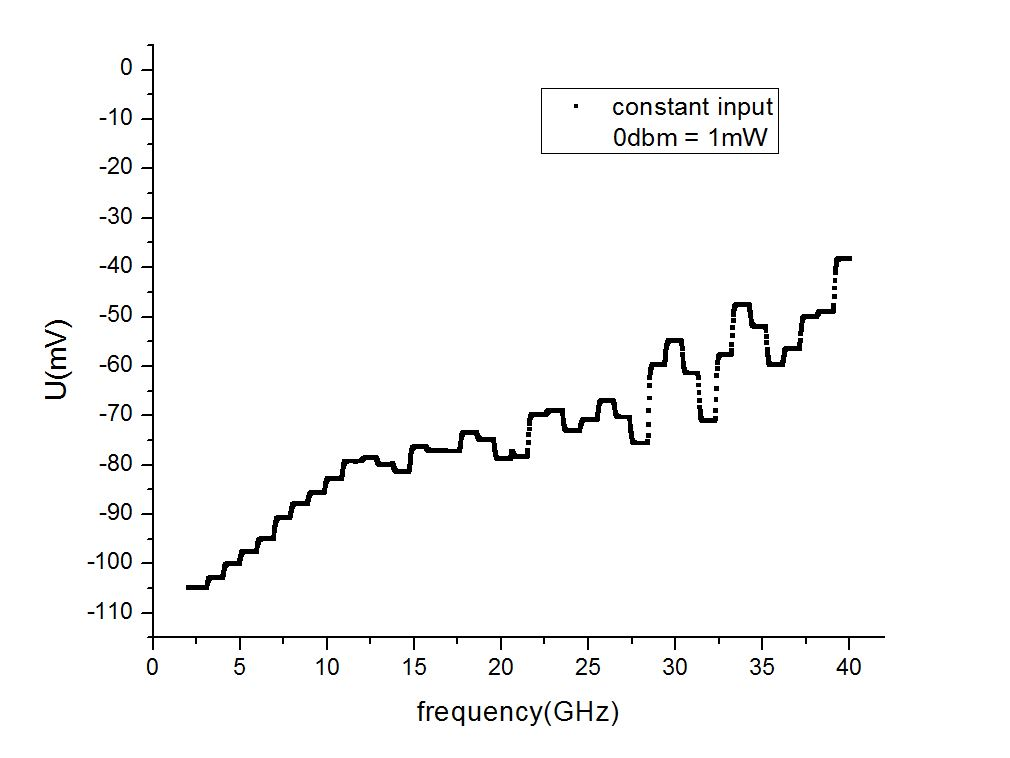
\includegraphics[width=\linewidth]{figures/spec.JPG}
     \label{spec}
   \end{minipage}
   \begin {minipage}{0.49\textwidth}
     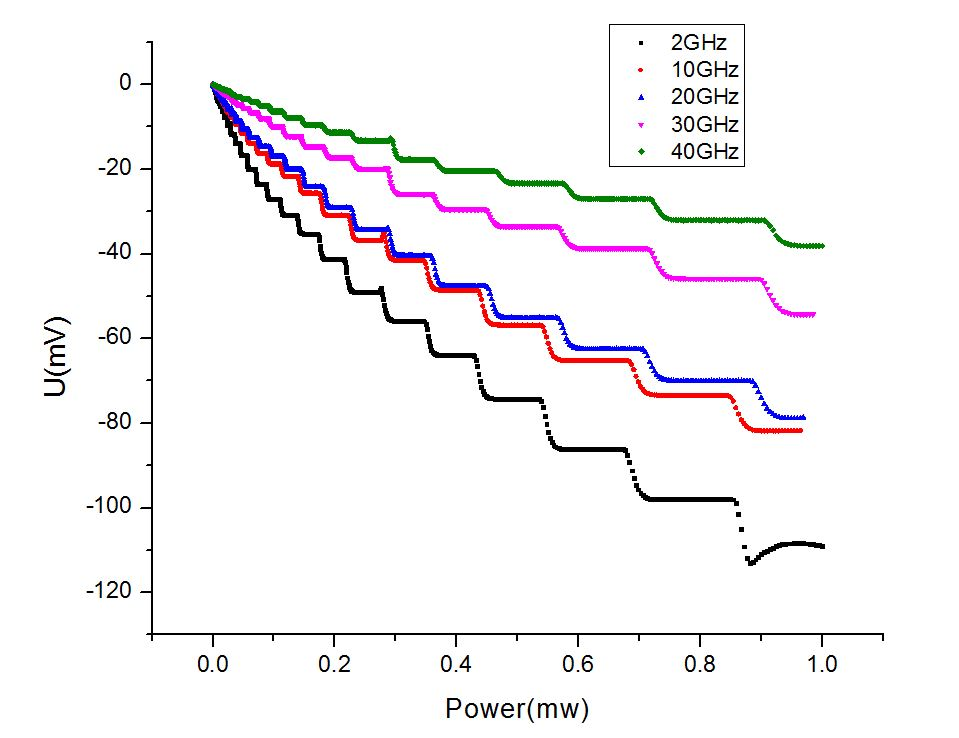
\includegraphics[width=\linewidth]{figures/multifre.JPG}
     \label{multifre}
   \end{minipage}
   \caption{setup calibration}
\end{figure}


 
This means our setup works better at lower frequencies. 
Actually, if we do a polynomial fitting (\figureref{cali_fitting}) at $\SI{2}{\giga \hertz}$, the result is very satisfying. 
 

\begin{figure}[!htb]\centering
   \begin{minipage}{0.49\textwidth}
     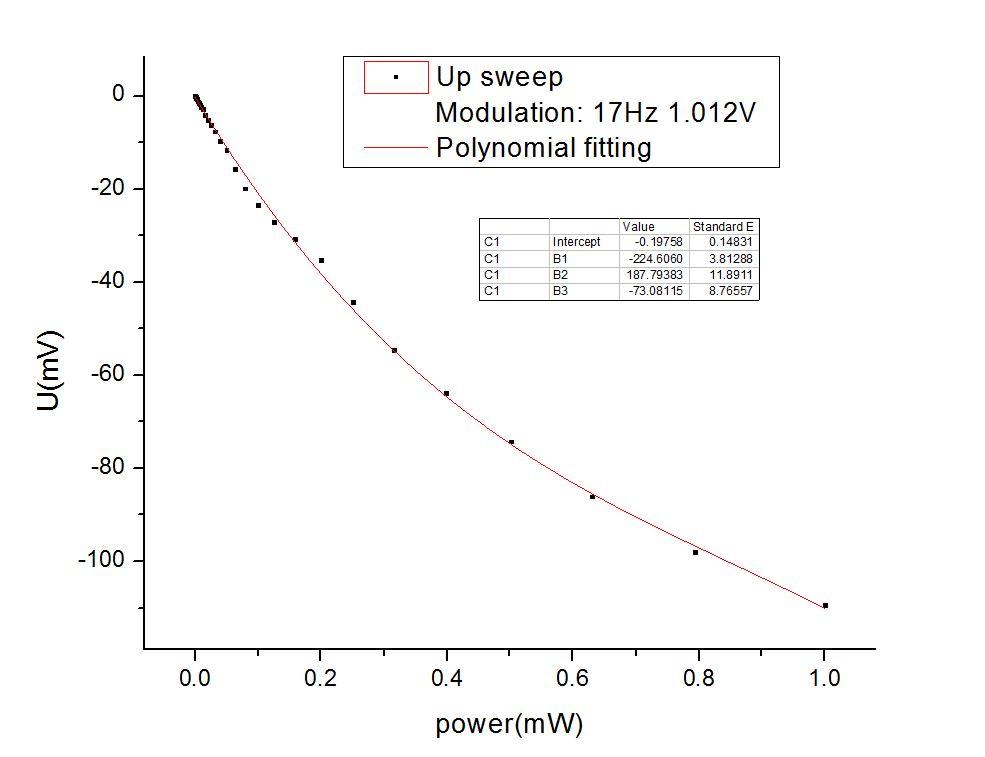
\includegraphics[width=\linewidth]{figures/cali_fitting.JPG}
     \caption{Polynomial fitting}\label{cali_fitting}
   \end{minipage}
   \begin {minipage}{0.49\textwidth}
     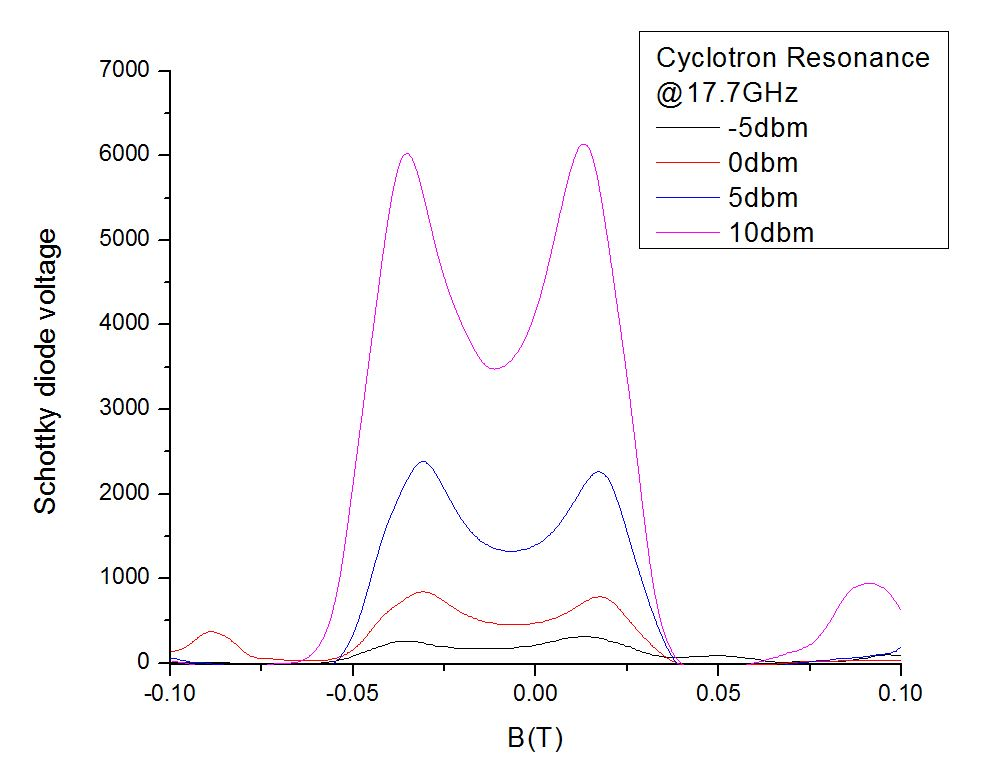
\includegraphics[width=\linewidth]{figures/CRpowerdep.JPG}
     \caption{CR pretest}\label{crpowerdep}
   \end{minipage}
\end{figure}


Therefore, it is quite convincing that the negative voltage measured by the detector has a polynomial dependence with the input power intensity.
 
 


 
 
\section{Cyclotron resonance pretest}\label{Cyclotron}

CR is a good test for this setup at larger frequencies so that electrons can go at least one circle before any collision and the peaks are separated far enough to resolve. 
\figureref{crpowerdep} shows symmetric CR peaks appear when magnetic field is swept and the signal is higher with larger input power.  









\section{Improvement underway}\label{Improvement}

Though CR can be resolved clearly, we are unable to see authentic repeatable edge state absorption peaks
and there are sudden bursts of noise due to reflection and thermal fluctuation.
Possible reasons are N-grease being too thick for electric field to probe edge state or even current equipment precision being not high enough to resolve the edge state absorption. 
We've come up with new ideas to improve the situation and new design is ready to be manufactured. 





\chapter{Summary}\label{summary}

The main theme is using microwave to detect various resonance phenomenon including CR, ESR, GR, and edge state.
We developed tools for different purposes such as transport, thermal and absorption measurement setups.
We successfully resolved CR on 2DEG, GR on 2DEG, ESR on DDPH and are working on detecting edge state resonance. 



\appendix

\bibliographystyle{ieeetr}
\bibliography{RPR}

\end{document}
